\documentclass[10pt]{article}
\usepackage{latexsym}
\usepackage{natbib}
\usepackage{graphicx}
\usepackage{caption}
\usepackage{subcaption}
\usepackage{listings}

\title{Homework 2: Independent Component Analysis}
\author{Name: Shun Zhang\\
Email address: \texttt{jensen.zhang@utexas.edu}\\
EID: \texttt{sz4554}}
\date{}

\begin{document}
\maketitle

\section{Independent Component Analysis}

In this report, I applied Independent Component Analysis on Blind Source
Separation problem.

\section{Experiment}

\begin{figure}
\centering
\begin{subfigure}[b]{0.49\textwidth}
	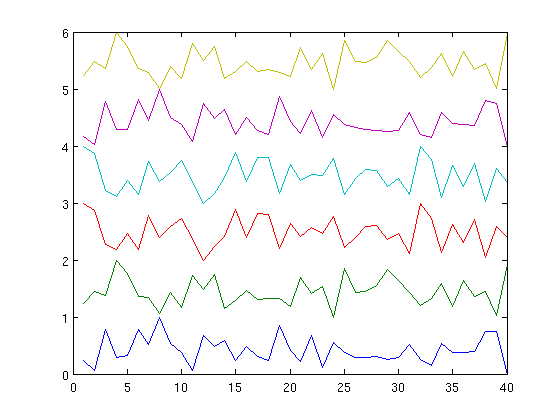
\includegraphics[width=\textwidth]{rep2.png}
\end{subfigure}
\begin{subfigure}[b]{0.49\textwidth}
	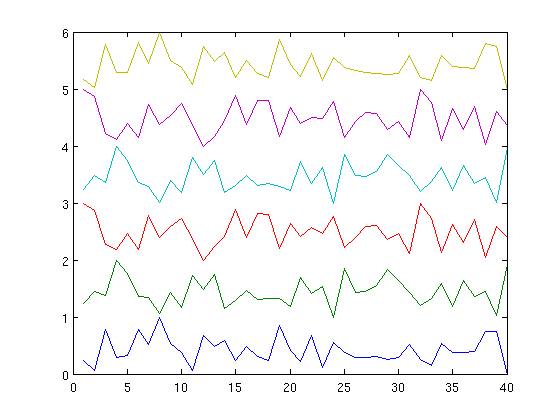
\includegraphics[width=\textwidth]{rep3.png}
\end{subfigure}
\caption{The bottom 3 lines are original signals from
\texttt{icaTest.mat}. The top 3 lines are reconstructed signals with
$\eta = 0.01$ and 1000000 iterations. The results are scaled into $[0, 1]$
interval. This experiment is repeated twice.  The results are in the
figures shown above. The result can be permutation of the original sources.
In the left figure, the mapping is 0-4, 1-5, 2-3. While in the right one,
the mapping is 0-5, 1-3, 2-4.}
\label{fig:rep}
\end{figure}

\begin{figure}
\centering
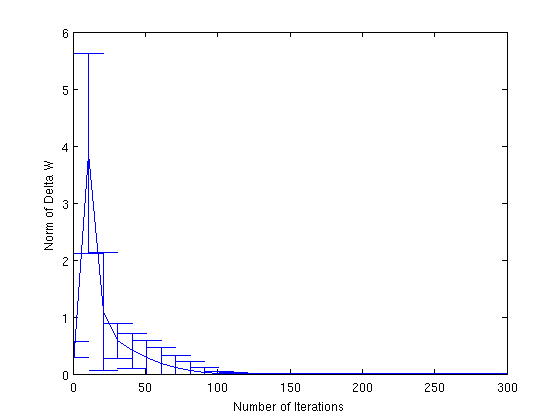
\includegraphics[width=.6\textwidth]{detW.png}
\caption{$\Delta W$ over number of iterations. Average of 5 runs. The
length of vertical bars is $\sigma$ assmuing Gaussian distribution of data
points at each iteration.}
\label{fig:detW}
\end{figure}

Frobenius Norm.

\section{Discussion}

\section{Conclusion}

\end{document}
